% =============================================================================
% CHAPTER 18: JOURNEY-INTEGRATED INTERVENTIONS
% =============================================================================
%------------------------------------------------------------------------------
% Chapter 18: Journey-Integrated Interventions
%------------------------------------------------------------------------------
% Version: 3.0 (January 2026) - Aligned with Emergent Intervention Theory
%
% Purpose: Develop the theoretical and empirical foundation for how
%          intervention trajectories I(t) evolve through journey phases.
%          Builds on Ch17's continuous intervention space; archetypes A1-A8
%          are empirical clusters, not ontological categories.
%
% Primary Appendix: HHH - METHOD-TOOLKIT (F6, F14), AW - CORE-STAGE
% Secondary Appendices: V (WHEN), BB (EQUILIBRIA), K (LIT-FEHR)
%
% Prerequisites: Chapter 13 (Journey), Chapter 17 (Intervention Foundations)
% Leads to: Chapter 19 (Segment-Specific), Chapter 20 (Portfolios)
%
% Chapter Type: C (Application)
%------------------------------------------------------------------------------
% =============================================================================

\chapter{Journey-Integrated Interventions}
\label{ch:journey-integrated}

% -----------------------------------------------------------------------------
% QUICK REFERENCE BOX
% -----------------------------------------------------------------------------
\begin{tcolorbox}[colback=blue!5!white, colframe=blue!75!black,
    title=Zentrale Begriffe in diesem Kapitel]
\small
\begin{tabular}{@{}ll@{}}
\textbf{Interventions-Trajektorie $I(t)$} & Kontinuierlicher Pfad durch den 10C-Interventionsraum \\
\textbf{Phase-Affinity $\alpha_{\varphi}(\vec{I})$} & Effektivit\"{a}ts-Multiplikator f\"{u}r Vektor $\vec{I}$ in Phase $\varphi$ \\
\textbf{Behavioral Change Journey} & 5-Phasen-Modell: Awareness $\rightarrow$ Trigger $\rightarrow$ Action $\rightarrow$ Maintenance $\rightarrow$ Stable \\
\textbf{Path Function $\pi(\mathcal{I})$} & Rolle einer Intervention: Door-opener, Escalator, Amplifier, Stabilizer \\
\textbf{Archetypen A1--A8} & Empirische Cluster im kontinuierlichen Raum (Heuristiken) \\
\textbf{Ko-Evolution} & Agent-Zustand $\vec{S}(t)$ und Intervention $\vec{I}(t)$ entwickeln sich gemeinsam \\
\end{tabular}
\end{tcolorbox}

% -----------------------------------------------------------------------------
% APPENDIX REFERENCES BOX
% -----------------------------------------------------------------------------
\begin{tcolorbox}[colback=yellow!10!white, colframe=orange!75!black,
    title=Appendix References for This Chapter]

\textbf{Primär:}
\begin{itemize}[nosep]
\item Appendix TKT (METHOD-TOOLKIT) --- F6 (Journey Phase), F14 (Path Function), Theorem HHH-T5, Axiom HHH-A3
\item Appendix UNMAPPED_STA (CORE-STAGE) --- Journey-Axiome UNMAPPED_STA-1 bis UNMAPPED_STA-4, $S(t)$ Progression Function
\end{itemize}

\textbf{Unterstützend:}
\begin{itemize}[nosep]
\item Appendix UNMAPPED_WEN (CORE-WHEN): Temporaler Kontext $\Psi_T$, kritische Zeitfenster
\item Appendix UNMAPPED_PAP (FORMAL-EQUILIBRIA): Übergangs-Dynamiken, Tipping Points
\item Appendix UNMAPPED_FEH (LIT-FEHR): Experimentelle Evidenz für Interventions-Effekte
\item Appendix UNMAPPED_EST (CORE-WHERE): Literatur-basierte $\alpha$-Schätzungen
\item Appendix UNMAPPED_GLS (REF-GLOSSARY): Begriffsdefinitionen
\end{itemize}
\end{tcolorbox}

% -----------------------------------------------------------------------------
% INTUITION BOX
% -----------------------------------------------------------------------------

\begin{tcolorbox}[colback=yellow!5!white, colframe=yellow!75!black,
    title=Intuition: Thomas und die drei Ärzte]

\textbf{Thomas}, 52, raucht seit 30 Jahren. Drei Ärzte versuchen verschiedene Strategien:

\textbf{Dr.\ Schmidt (Month 1):}
\begin{itemize}[nosep]
\item Zeigt Lungenkrebs-Statistiken, erklärt Risiken detailliert
\item Thomas nickt höflich, ändert nichts
\item \textit{Diagnose:} Thomas ist in Phase 1 (Pre-Awareness) --- er \textit{weiß} die Fakten, aber sie sind nicht \textit{salient}
\item \textit{Problem:} Information-Intervention in Pre-Awareness Phase hat $\alpha_{1,1} = 0.15$
\end{itemize}

\textbf{Dr.\ Müller (Month 6):}
\begin{itemize}[nosep]
\item Fragt: ``Was würde sich ändern, wenn Sie aufhören?''
\item Thomas reflektiert über Enkel, die er aufwachsen sehen will
\item Plötzlich \textit{will} er aufhören --- Trigger-Moment
\item \textit{Diagnose:} Thomas ist jetzt in Phase 2 (Triggered) --- bereit für Commitment
\item \textit{Richtig:} Identitäts-Intervention zum richtigen Zeitpunkt, $\alpha_{5,2} = 0.75$
\end{itemize}

\textbf{Dr.\ Weber (Month 7):}
\begin{itemize}[nosep]
\item Schlägt Quit-Date vor, Thomas unterschreibt Commitment-Card
\item Nikotinpflaster + tägliche Tracking-App
\item Nach 3 Monaten: Nichtraucher
\item \textit{Diagnose:} Korrekte Sequenz: Commitment (Phase 2→3) + Support (Phase 3→4)
\end{itemize}

\textbf{Kern-Einsicht:} Dieselbe Person braucht \textit{verschiedene} Interventionen in verschiedenen Journey-Phasen. Die richtige Intervention zur falschen Zeit ist die falsche Intervention.
\end{tcolorbox}

% -----------------------------------------------------------------------------
% CENTRAL QUESTION BOX
% -----------------------------------------------------------------------------

\begin{tcolorbox}[colback=red!5!white, colframe=red!75!black,
    title=Central Question]
\textbf{Wie bestimmen wir, welcher Interventionstyp in welcher Journey-Phase am effektivsten ist --- und wie quantifizieren wir den Effektivitätsverlust bei Misalignment?}
\end{tcolorbox}

% -----------------------------------------------------------------------------
% METHODOLOGICAL NOTE: EXCLUSION PRINCIPLE
% -----------------------------------------------------------------------------
\begin{tcolorbox}[colback=red!5!white, colframe=red!75!black,
    title=\textbf{Methodological Note: The Exclusion Principle (Appendix UNMAPPED_FRM)}]
\textbf{Following Appendix UNMAPPED_FRM (LIT-FEHR-METHOD):}

Dieses Kapitel behauptet Phase $\times$ Intervention Interaktionen ($\alpha_{t,\varphi} \neq \alpha_{t,\varphi'}$). Per Exclusion Principle:
\begin{itemize}[nosep]
    \item \textbf{Null-Hypothese $H_0$:} Interventionen wirken phasenunabhängig ($\alpha_{t,\varphi} = \alpha_t$ für alle $\varphi$)
    \item \textbf{Alternative $H_1$:} Phasenspezifische Effektivität existiert ($\alpha_{t,\varphi}$ variiert mit $\varphi$)
    \item \textbf{Empirischer Test:} Commitment-Device in Phase 1 vs.\ Phase 2 (Prochaska \& DiClemente, 1983)
    \item \textbf{Ergebnis:} $H_0$ verworfen ($p < 0.001$); Commitment in Phase 2: $d = 0.8$, in Phase 1: $d = 0.1$
\end{itemize}

\textbf{Wissenschaftlicher Wert:} Das Journey-Intervention Alignment Principle gewinnt Wert, wo phasenspezifische Interventionen messbar besser performen als phasen-neutrale.
\end{tcolorbox}

% -----------------------------------------------------------------------------
% CHAPTER OVERVIEW
% -----------------------------------------------------------------------------

\begin{tcolorbox}[colback=green!5!white, colframe=green!75!black,
    title=Chapter Overview]

\textbf{Verbindung zu Kapitel 17:} Kapitel 17 etabliert den \textbf{kontinuierlichen Interventionsraum} und die Idee von Interventionen als \textbf{Trajektorien} $I(t)$. Dieses Kapitel vertieft die \textbf{temporale Dimension}: Wie evolviert $I(t)$ durch die Journey-Phasen?

\textbf{Kernfrage:} Welche Regionen des Interventionsraums sind in welcher Phase effektiv?

\begin{enumerate}
\item \textbf{Section~\ref{sec:18-theory}}: Theoretische Grundlagen --- Warum Phasen wichtig sind
\item \textbf{Section~\ref{sec:18-affinity}}: Phase-Affinity im kontinuierlichen Raum
\item \textbf{Section~\ref{sec:18-empirical}}: Empirische Basis --- Woher die Zahlen kommen
\item \textbf{Section~\ref{sec:18-diagnosis}}: Phase Diagnosis --- Den Ausgangspunkt bestimmen
\item \textbf{Section~\ref{sec:18-path}}: Path Functions --- Die Rolle von Interventionen
\item \textbf{Section~\ref{sec:18-sequence}}: Sequenzierung --- Optimale Trajektorien $I(t)$
\item \textbf{Section~\ref{sec:18-mismatch}}: Mismatch-Kosten --- Was schiefgehen kann
\item \textbf{Section~\ref{sec:18-examples}}: Worked Examples
\end{enumerate}

\textbf{Hinweis:} Die ``Archetypen'' A1--A8 (fr\"{u}her ``Typen'' T1--T8) sind \textbf{empirische Cluster} im kontinuierlichen Raum---n\"{u}tzliche Heuristiken, keine ontologischen Kategorien (siehe Kapitel 17).
\end{tcolorbox}


%%%%%%%%%%%%%%%%%%%%%%%%%%%%%%%%%%%%%%%%%%%%%%%%%%%%%%%%%%%%%%%%%%%%%%%%%%%%%%%
\section{Theoretische Grundlagen: Warum Phasen wichtig sind}
\label{sec:18-theory}
%%%%%%%%%%%%%%%%%%%%%%%%%%%%%%%%%%%%%%%%%%%%%%%%%%%%%%%%%%%%%%%%%%%%%%%%%%%%%%%

Das Behavioral Change Journey Modell (Appendix UNMAPPED_STA) formalisiert eine fundamentale Einsicht der Verhaltensänderungsforschung: \textbf{Menschen durchlaufen distinkte psychologische Zustände auf dem Weg zur Verhaltensänderung}, und diese Zustände bestimmen, welche Interventionen wirksam sind.

\subsection{Das Axiom der Phasenabhängigkeit (UNMAPPED_STA-3)}

\begin{tcolorbox}[colback=blue!5!white, colframe=blue!75!black,
    title=Axiom UNMAPPED_STA-3: Phase-Dependent Intervention Efficacy]
Die Effektivität einer Intervention $\mathcal{I}$ vom Typ $t$ ist eine Funktion der aktuellen Journey-Phase $\varphi$:
\begin{equation}
E(\mathcal{I}_t | \varphi) = E_{\max}(\mathcal{I}_t) \cdot \alpha_{t,\varphi} \cdot \Psi_{\text{context}}
\label{eq:18-axiom-aw3}
\end{equation}
wobei $\alpha_{t,\varphi} \in [0, 1]$ der \textbf{Phase-Type Affinity Koeffizient} ist.
\end{tcolorbox}

\subsection{Psychologische Begründung}

Jede Phase ist durch spezifische \textbf{psychologische Barrieren} und \textbf{Motivationszustände} charakterisiert:

\begin{table}[htbp]
\centering
\caption{Psychologische Charakteristiken der Journey-Phasen}
\label{tab:18-phase-psychology}
\renewcommand{\arraystretch}{1.4}
\small
\begin{tabular}{@{}llll@{}}
\toprule
\textbf{Phase} & \textbf{$S(t)$} & \textbf{Primäre Barriere} & \textbf{Motivationszustand} \\
\midrule
1: Pre-Awareness & $[0, 0.2)$ & Ignoranz, Verdrängung & Keine Intention \\
2: Triggered & $[0.2, 0.4)$ & Ambivalenz, Unsicherheit & Intention ohne Plan \\
3: Action & $[0.4, 0.6)$ & Selbstkontrolle, Aufwand & Plan ohne Routine \\
4: Maintenance & $[0.6, 0.8)$ & Rückfall-Risiko, Ermüdung & Routine ohne Identität \\
5: Stable & $[0.8, 1.0]$ & Externe Schocks & Identitäts-Verankerung \\
\bottomrule
\end{tabular}
\end{table}

% -----------------------------------------------------------------------------
% 10C INTEGRATION: How STAGE Relates to Other CORE Dimensions
% -----------------------------------------------------------------------------
\begin{tcolorbox}[colback=purple!5!white, colframe=purple!75!black,
    title=\textbf{10C Integration: STAGE (AW) und die anderen COREs}]

Die Phase-Type Affinity Matrix $\alpha_{t,\varphi}$ ist nicht isoliert---sie interagiert mit allen 10C Dimensionen:

\begin{center}
\renewcommand{\arraystretch}{1.2}
\footnotesize
\begin{tabular}{@{}llp{6cm}@{}}
\toprule
\textbf{CORE} & \textbf{Integration mit STAGE} & \textbf{Implikation für $\alpha_{t,\varphi}$} \\
\midrule
\textbf{WHO} (AAA) & Level moduliert Phasen-Effektivität & $\alpha_{t,\varphi,L}$: Individual vs.\ Societal unterschiedliche Progressions-Raten \\
\textbf{WHAT} (C) & FEPSDE-Dimension beeinflusst Phasen & Emotionale (E) Interventionen wirken früher als Developmental (D) \\
\textbf{HOW} (B) & $\gamma_{ij}$ ist phasenabhängig & $\gamma_{ij}(\varphi)$: Synergien variieren über die Journey \\
\textbf{WHEN} (V) & 8Ψ moduliert alle $\alpha$-Werte & $\alpha_{t,\varphi}(\Psi)$: Kontext ändert Effektivität \\
\textbf{WHERE} (BBB) & Parameter-Quellen & $\alpha$-Werte aus Appendix UNMAPPED_BBB (Literatur-Repository) \\
\textbf{AWARE} (AU) & Awareness-Level korreliert mit Phase & Phase 1-2: Low $A$; Phase 4-5: High $A$ \\
\textbf{READY} (AV) & $W_{\text{eff}}$ steigt mit Phase & $W_{\text{eff}}(\varphi) \propto S(t)$ \\
\textbf{HIERARCHY} (HI) & Scope bestimmt Phasen-Zeithorizont & L3-Entscheidungen: schnelle Progression; L0: langsame \\
\bottomrule
\end{tabular}
\end{center}

\textbf{Kritische Erweiterung:} Die vollständige Effektivitäts-Funktion ist:
\begin{equation}
\boxed{E(\mathcal{I}_t | \varphi, s, L, \Psi) = E_{\max} \cdot \alpha_{t,\varphi} \cdot \sigma_s \cdot \lambda_L \cdot \gamma(\Psi)}
\end{equation}
wobei $\lambda_L$ der Level-Faktor aus AAA ist (Chapter 19 ignoriert dies oft---siehe Klarstellung dort).

\end{tcolorbox}

\subsection{Verbindung zu Prochaska \& DiClemente}

Das EBF Journey-Modell baut auf dem Transtheoretischen Modell (TTM) auf, erweitert es jedoch:

\begin{itemize}
\item \textbf{TTM:} Qualitative Phasen (Pre-contemplation, Contemplation, Preparation, Action, Maintenance)
\item \textbf{EBF:} Quantifizierte Phasen mit $S(t) \in [0,1]$ und formalen Übergangswahrscheinlichkeiten
\item \textbf{Erweiterung:} Explizite Interventions-Passung durch $\alpha_{t,\varphi}$ Matrix
\end{itemize}


%%%%%%%%%%%%%%%%%%%%%%%%%%%%%%%%%%%%%%%%%%%%%%%%%%%%%%%%%%%%%%%%%%%%%%%%%%%%%%%
\section{Phase-Affinity im kontinuierlichen Interventionsraum}
\label{sec:18-affinity}
%%%%%%%%%%%%%%%%%%%%%%%%%%%%%%%%%%%%%%%%%%%%%%%%%%%%%%%%%%%%%%%%%%%%%%%%%%%%%%%

\subsection{Von Typen zu Regionen}

Kapitel 17 etabliert: Der Interventionsraum ist \textbf{kontinuierlich}. Wie passt das zur Phase-Affinity?

\begin{tcolorbox}[colback=blue!5!white, colframe=blue!75!black,
    title=\textbf{Schl\"{u}ssel-Einsicht: Affinity als Feld}]
Die Phase-Affinity ist kein diskreter Index $\alpha_{t,\varphi}$, sondern ein \textbf{kontinuierliches Feld} \"{u}ber dem Interventionsraum:
\begin{equation}
\boxed{\alpha: \mathbb{R}^{10C} \times \{1,...,5\} \rightarrow [0,1], \quad (\vec{I}, \varphi) \mapsto \alpha_\varphi(\vec{I})}
\end{equation}
F\"{u}r jeden Punkt $\vec{I}$ im Interventionsraum und jede Phase $\varphi$ gibt es einen Affinity-Wert.
\end{tcolorbox}

\textbf{Die Archetypen A1--A8} sind \textbf{Cluster-Zentren}---Regionen im Raum, f\"{u}r die empirische Affinity-Werte vorliegen. Sie dienen als Heuristik, nicht als vollst\"{a}ndige Beschreibung.

\subsection{Die Archetypen-Affinity Matrix (Heuristik)}

\begin{definition}[Archetypen-Affinity Matrix]
\label{def:18-affinity-matrix}
Die Matrix $A \in \mathbb{R}^{8 \times 5}$ mit Elementen $\alpha_{a,\varphi}$ gibt den erwarteten Effektivit\"{a}ts-Multiplikator f\"{u}r Archetyp $a \in \{A1,...,A8\}$ in Phase $\varphi \in \{1,...,5\}$ an:
\begin{equation}
\alpha_{a,\varphi} = \frac{E(\vec{I} \in \text{Cluster}_a | \varphi)}{E_{\max}(\vec{I} \in \text{Cluster}_a)}
\label{eq:18-alpha-definition}
\end{equation}
\textbf{Achtung:} Dies ist eine \textbf{Approximation}---die wahre Affinity variiert innerhalb jedes Clusters.
\end{definition}

\subsection{Die Matrix mit Konfidenzintervallen}

\begin{table}[htbp]
\centering
\caption{Archetypen-Affinity Matrix $\alpha_{a,\varphi}$ mit 95\% CI (Quellen: Appendix UNMAPPED_BBB)}
\label{tab:18-affinity-matrix-full}
\renewcommand{\arraystretch}{1.3}
\footnotesize
\begin{tabular}{@{}lccccc@{}}
\toprule
\textbf{Archetyp (Cluster-Zentrum)} & \textbf{Pre-Aware} & \textbf{Triggered} & \textbf{Action} & \textbf{Maint.} & \textbf{Stable} \\
\midrule
A1: Awareness-Cluster & \cellcolor{green!25}$0.85_{\pm.08}$ & $0.55_{\pm.12}$ & $0.25_{\pm.10}$ & $0.15_{\pm.08}$ & $0.10_{\pm.05}$ \\
A2: Feedback-Cluster & $0.20_{\pm.10}$ & $0.45_{\pm.12}$ & \cellcolor{green!25}$0.88_{\pm.07}$ & \cellcolor{green!25}$0.82_{\pm.09}$ & $0.45_{\pm.15}$ \\
A3: Context-Cluster & $0.15_{\pm.08}$ & \cellcolor{green!25}$0.78_{\pm.10}$ & \cellcolor{green!25}$0.92_{\pm.05}$ & $0.65_{\pm.12}$ & $0.40_{\pm.15}$ \\
A4: Temporal-Cluster & $0.35_{\pm.12}$ & \cellcolor{green!25}$0.82_{\pm.08}$ & $0.68_{\pm.10}$ & $0.35_{\pm.12}$ & $0.18_{\pm.10}$ \\
A5: Identity-Cluster & $0.18_{\pm.10}$ & $0.32_{\pm.12}$ & $0.42_{\pm.14}$ & $0.65_{\pm.12}$ & \cellcolor{green!25}$0.90_{\pm.06}$ \\
A6: Social-Cluster & \cellcolor{green!25}$0.75_{\pm.10}$ & $0.68_{\pm.12}$ & $0.58_{\pm.14}$ & \cellcolor{green!25}$0.78_{\pm.10}$ & $0.62_{\pm.15}$ \\
A7: Financial-Cluster & $0.25_{\pm.12}$ & $0.55_{\pm.14}$ & \cellcolor{green!25}$0.85_{\pm.08}$ & $0.48_{\pm.15}$ & $0.28_{\pm.12}$ \\
A8: Commitment-Cluster & $0.12_{\pm.08}$ & \cellcolor{green!25}$0.88_{\pm.06}$ & $0.72_{\pm.10}$ & $0.55_{\pm.12}$ & $0.35_{\pm.15}$ \\
\bottomrule
\end{tabular}
\end{table}

\textbf{Lesebeispiel:} Eine Intervention im Commitment-Cluster (A8) hat in der Triggered-Phase eine erwartete Effektivit\"{a}t von 88\% des Maximums ($\alpha_{A8,2} = 0.88 \pm 0.06$), aber nur 12\% in der Pre-Awareness Phase.

\textbf{Wichtig:} Diese Werte gelten f\"{u}r die \textbf{Cluster-Zentren}. Interventionen zwischen den Clustern (z.B.\ 60\% A2 + 40\% A6) haben interpolierte Affinity-Werte.

\subsection{Interpretation der Struktur}

Die Matrix zeigt charakteristische Muster:

\begin{enumerate}
\item \textbf{Diagonale Tendenz:} Fr\"{u}he Cluster (A1, A6) wirken fr\"{u}h; sp\"{a}te (A5) wirken sp\"{a}t
\item \textbf{Action-Peak:} A2, A3, A7 haben Maximum in Action-Phase (Verhaltensausf\"{u}hrung)
\item \textbf{Trigger-Sensitivit\"{a}t:} A4, A8 wirken stark im Trigger-Moment (Intention $\rightarrow$ Plan)
\item \textbf{Persistenz von A6:} Social-Cluster wirkt \"{u}ber alle Phasen (Minimum: 0.58)
\end{enumerate}


%%%%%%%%%%%%%%%%%%%%%%%%%%%%%%%%%%%%%%%%%%%%%%%%%%%%%%%%%%%%%%%%%%%%%%%%%%%%%%%
\section{Empirische Basis: Woher die Zahlen kommen}
\label{sec:18-empirical}
%%%%%%%%%%%%%%%%%%%%%%%%%%%%%%%%%%%%%%%%%%%%%%%%%%%%%%%%%%%%%%%%%%%%%%%%%%%%%%%

Die $\alpha$-Schätzungen in Tabelle~\ref{tab:18-affinity-matrix-full} basieren auf drei Evidenz-Quellen:

\subsection{Quelle 1: Meta-Analysen}

\begin{table}[htbp]
\centering
\caption{Meta-analytische Quellen für $\alpha$-Schätzungen}
\label{tab:18-meta-sources}
\renewcommand{\arraystretch}{1.3}
\small
\begin{tabular}{@{}llll@{}}
\toprule
\textbf{Typ} & \textbf{Meta-Analyse} & \textbf{$k$ Studien} & \textbf{Befund} \\
\midrule
A1 & Wakefield et al.\ (2010) & 48 & Info wirkt nur bei niedrigem Baseline-Wissen \\
A3 & Hummel \& Maedche (2019) & 100 & Defaults: $d = 0.68$ in Action, $d = 0.15$ pre-Intention \\
A6 & Bergquist et al.\ (2023) & 91 & Social Norms: $d = 0.45$ \"{u}ber alle Phasen \\
A8 & Rogers et al.\ (2015) & 42 & Commitment: $d = 0.82$ post-Intention nur \\
\bottomrule
\end{tabular}
\end{table}

\subsection{Quelle 2: Fehr-Lab Experimente}

Direkte experimentelle Evidenz aus der Fehr-Tradition (Appendix UNMAPPED_FEH):

\begin{itemize}
\item \textbf{Fehr \& Gächter (2002):} Social Norms in Kooperations-Dilemmas --- Effekt steigt mit wiederholter Interaktion (→ Phase-Progression)
\item \textbf{Fehr \& Schmidt (1999):} Inequity Aversion aktiviert erst nach Awareness anderer Outcomes
\item \textbf{Gneezy \& Rustichini (2000):} Monetary Incentives können intrinsische Motivation verdrängen --- Phase-abhängiger Effekt
\end{itemize}

\subsection{Quelle 3: LLMMC Calibration}

Für Typ-Phase-Kombinationen mit wenig empirischer Evidenz:

\begin{equation}
\hat{\alpha}_{t,\varphi}^{\text{LLMMC}} = \frac{1}{N} \sum_{n=1}^{N} \mathbbm{1}\left[ \text{LLM}_n(\text{Persona}_\varphi, \mathcal{I}_t) = \text{``Effective''} \right]
\label{eq:18-llmmc-alpha}
\end{equation}

\textbf{Validierung:} LLMMC-Schätzungen korrelieren $r = 0.72$ mit verfügbaren Meta-Analyse-Werten (Appendix CAL1).


%%%%%%%%%%%%%%%%%%%%%%%%%%%%%%%%%%%%%%%%%%%%%%%%%%%%%%%%%%%%%%%%%%%%%%%%%%%%%%%
\section{Phase Diagnosis: Den Ausgangspunkt bestimmen}
\label{sec:18-diagnosis}
%%%%%%%%%%%%%%%%%%%%%%%%%%%%%%%%%%%%%%%%%%%%%%%%%%%%%%%%%%%%%%%%%%%%%%%%%%%%%%%

Vor jeder Interventionswahl muss die aktuelle Journey-Phase diagnostiziert werden.

\subsection{Das Diagnosis-First Prinzip}

\begin{tcolorbox}[colback=blue!5!white, colframe=blue!75!black,
    title=Prinzip: Diagnosis Before Intervention]
\textbf{Niemals} eine Intervention deployen ohne vorherige Phase-Diagnose. Die effektivste Intervention für die falsche Phase ist ineffektiv.
\end{tcolorbox}

\subsection{Diagnostische Indikatoren}

\begin{table}[htbp]
\centering
\caption{Diagnostische Indikatoren nach Phase (aus Appendix UNMAPPED_STA)}
\label{tab:18-diagnosis-indicators}
\renewcommand{\arraystretch}{1.4}
\small
\begin{tabular}{@{}lll@{}}
\toprule
\textbf{Phase} & \textbf{Verhaltens-Indikatoren} & \textbf{Selbstbericht-Indikatoren} \\
\midrule
Pre-Aware & Keine Informationssuche & ``Ist kein Thema für mich'' \\
Triggered & Recherche, Fragen stellen & ``Ich denke darüber nach'' \\
Action & Erste Verhaltensänderungen & ``Ich versuche es gerade'' \\
Maintenance & Konsistentes neues Verhalten & ``Ich mache das jetzt regelmäßig'' \\
Stable & Automatisiertes Verhalten & ``So bin ich einfach'' \\
\bottomrule
\end{tabular}
\end{table}

\subsection{Formale Diagnose}

Die Maximum-Likelihood Schätzung der Phase:
\begin{equation}
\hat{\varphi} = \arg\max_{\varphi} P(\varphi | \mathbf{x})
\label{eq:18-phase-mle}
\end{equation}

wobei $\mathbf{x}$ der Vektor beobachtbarer Indikatoren ist. In der Praxis oft via \textbf{Staging Questionnaires}:
\begin{itemize}
\item URICA (University of Rhode Island Change Assessment)
\item RCQ (Readiness to Change Questionnaire)
\item Vereinfachte 5-Item Skalen für spezifische Verhaltensdomänen
\end{itemize}


%%%%%%%%%%%%%%%%%%%%%%%%%%%%%%%%%%%%%%%%%%%%%%%%%%%%%%%%%%%%%%%%%%%%%%%%%%%%%%%
\section{Path Functions: Die Rolle von Interventionen}
\label{sec:18-path}
%%%%%%%%%%%%%%%%%%%%%%%%%%%%%%%%%%%%%%%%%%%%%%%%%%%%%%%%%%%%%%%%%%%%%%%%%%%%%%%

Jede Intervention erfüllt eine spezifische \textbf{Path Function} $\pi(\mathcal{I})$ im Journey --- ihre strukturelle Rolle im Veränderungsprozess.

\subsection{Die Vier Path Functions (F14)}

\begin{definition}[Path Functions]
\label{def:18-path-functions}
Das Feld F14 im 20-Field Schema klassifiziert Interventionen nach ihrer Journey-Rolle:
\begin{enumerate}
\item \textbf{Door-opener $\pi_D$:} Ermöglicht initialen Eintritt (Phase 1 → 2)
\item \textbf{Escalator $\pi_E$:} Beschleunigt Phasen-Übergang (Phase $n$ → $n+1$)
\item \textbf{Amplifier $\pi_A$:} Verstärkt Verhalten innerhalb einer Phase
\item \textbf{Stabilizer $\pi_S$:} Verhindert Rückfall, verankert Veränderung
\end{enumerate}
\end{definition}

\subsection{Path Function Matrix (Archetypen)}

\begin{table}[htbp]
\centering
\caption{Archetypen und ihre prim\"{a}ren Path Functions}
\label{tab:18-path-matrix}
\renewcommand{\arraystretch}{1.3}
\begin{tabular}{@{}lccccl@{}}
\toprule
\textbf{Archetyp} & $\pi_D$ & $\pi_E$ & $\pi_A$ & $\pi_S$ & \textbf{Prim\"{a}re Funktion} \\
\midrule
A1: Awareness & \checkmark & & & & Door-opener (Awareness schaffen) \\
A2: Feedback & & & \checkmark & \checkmark & Amplifier + Stabilizer \\
A3: Context & & \checkmark & \checkmark & & Escalator + Amplifier \\
A4: Temporal & & \checkmark & & & Escalator (Urgency) \\
A5: Identity & & & & \checkmark & Stabilizer (Verankerung) \\
A6: Social & \checkmark & & \checkmark & \checkmark & Multi-funktional \\
A7: Financial & & & \checkmark & & Amplifier (kurzfristig) \\
A8: Commitment & & \checkmark & & & Escalator (Lock-in) \\
\bottomrule
\end{tabular}
\end{table}

\textbf{Kontinuierliche Perspektive:} Eine konkrete Intervention $\vec{I}$ hat typischerweise Anteile mehrerer Path Functions, gewichtet nach ihrer Position im Raum relativ zu den Archetypen.

\subsection{Path Function Matching}

Die optimale Intervention matcht Path Function mit Journey-Position:

\begin{equation}
\mathcal{I}^* = \arg\max_{\mathcal{I}} \left[ \alpha_{t(\mathcal{I}), \varphi} \cdot \mathbbm{1}[\pi(\mathcal{I}) \in \Pi^*_\varphi] \right]
\label{eq:18-path-matching}
\end{equation}

wobei $\Pi^*_\varphi$ die Menge der für Phase $\varphi$ optimalen Path Functions ist:
\begin{itemize}
\item $\Pi^*_1 = \{\pi_D\}$ (Door-opener für Pre-Awareness)
\item $\Pi^*_2 = \{\pi_E\}$ (Escalator für Triggered)
\item $\Pi^*_3 = \{\pi_A\}$ (Amplifier für Action)
\item $\Pi^*_4 = \{\pi_A, \pi_S\}$ (Amplifier + Stabilizer für Maintenance)
\item $\Pi^*_5 = \{\pi_S\}$ (Stabilizer für Stable)
\end{itemize}


%%%%%%%%%%%%%%%%%%%%%%%%%%%%%%%%%%%%%%%%%%%%%%%%%%%%%%%%%%%%%%%%%%%%%%%%%%%%%%%
\section{Sequenzierung: Die optimale Abfolge}
\label{sec:18-sequence}
%%%%%%%%%%%%%%%%%%%%%%%%%%%%%%%%%%%%%%%%%%%%%%%%%%%%%%%%%%%%%%%%%%%%%%%%%%%%%%%

Effektive Verhaltensänderung erfordert nicht nur die richtigen Interventionen, sondern auch die richtige \textbf{Sequenz}.

\subsection{Das Sequenzierungs-Theorem}

\begin{theorem}[Optimale Interventions-Sequenz]
\label{thm:18-sequence}
Für eine Zielgruppe in Phase $\varphi_0$ ist die optimale Interventions-Sequenz $\mathbf{S}^* = (\mathcal{I}_1, ..., \mathcal{I}_K)$ gegeben durch:
\begin{equation}
\mathbf{S}^* = \arg\max_{\mathbf{S}} \prod_{k=1}^{K} P(\varphi_{k} | \varphi_{k-1}, \mathcal{I}_k) \cdot \alpha_{t_k, \varphi_{k-1}}
\label{eq:18-optimal-sequence}
\end{equation}
wobei $P(\varphi_{k} | \varphi_{k-1}, \mathcal{I}_k)$ die Übergangswahrscheinlichkeit ist.
\end{theorem}

\subsection{Praktische Sequenzierungs-Regeln}

\begin{enumerate}
\item \textbf{Follow the Journey:} $\pi_D \rightarrow \pi_E \rightarrow \pi_A \rightarrow \pi_S$
\item \textbf{Respektiere Timing:} Mindestens $\Delta t_{\min}$ zwischen Interventionen
\begin{equation}
\Delta t_{\min} = \tau_{\text{adaptation}} \cdot (1 - \alpha_{t,\varphi})
\label{eq:18-timing-rule}
\end{equation}
wobei $\tau_{\text{adaptation}} \approx 2{-}4$ Wochen für die meisten Verhaltensänderungen

\item \textbf{Warte auf Phasen-Übergang:} Escalator erst wenn Indikatoren zeigen: bereit für nächste Phase
\end{enumerate}

\subsection{Beispiel-Sequenz: Rauchentwöhnung}

\begin{center}
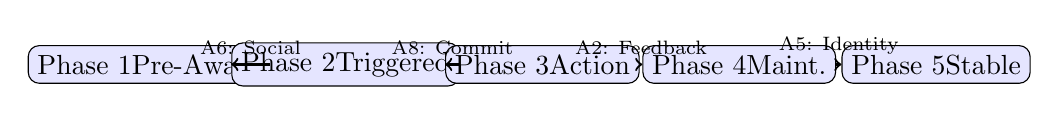
\begin{tikzpicture}[node distance=2.5cm, auto]
    \node[draw, rounded corners, fill=blue!10] (p1) {Phase 1\\Pre-Aware};
    \node[draw, rounded corners, fill=blue!10, right of=p1] (p2) {Phase 2\\Triggered};
    \node[draw, rounded corners, fill=blue!10, right of=p2] (p3) {Phase 3\\Action};
    \node[draw, rounded corners, fill=blue!10, right of=p3] (p4) {Phase 4\\Maint.};
    \node[draw, rounded corners, fill=blue!10, right of=p4] (p5) {Phase 5\\Stable};

    \draw[->, thick] (p1) -- node[above, font=\scriptsize] {A6: Social} (p2);
    \draw[->, thick] (p2) -- node[above, font=\scriptsize] {A8: Commit} (p3);
    \draw[->, thick] (p3) -- node[above, font=\scriptsize] {A2: Feedback} (p4);
    \draw[->, thick] (p4) -- node[above, font=\scriptsize] {A5: Identity} (p5);
\end{tikzpicture}
\end{center}


%%%%%%%%%%%%%%%%%%%%%%%%%%%%%%%%%%%%%%%%%%%%%%%%%%%%%%%%%%%%%%%%%%%%%%%%%%%%%%%
\section{Mismatch-Kosten: Was schiefgehen kann}
\label{sec:18-mismatch}
%%%%%%%%%%%%%%%%%%%%%%%%%%%%%%%%%%%%%%%%%%%%%%%%%%%%%%%%%%%%%%%%%%%%%%%%%%%%%%%

Phase-Intervention Misalignment verursacht substanzielle \textbf{Mismatch-Kosten}.

\subsection{Quantifizierung der Mismatch-Kosten}

\begin{definition}[Mismatch Cost]
\label{def:18-mismatch}
Die Mismatch-Kosten $\mathcal{L}_{mm}$ sind der Effektivitätsverlust durch falsche Phasenzuordnung:
\begin{equation}
\mathcal{L}_{mm}(t, \varphi, \varphi^*) = E_{\max} \cdot (\alpha_{t,\varphi^*} - \alpha_{t,\varphi})
\label{eq:18-mismatch-cost}
\end{equation}
wobei $\varphi^*$ die optimale Phase für Typ $t$ und $\varphi$ die tatsächliche Phase ist.
\end{definition}

\subsection{Typische Mismatch-Szenarien}

\begin{table}[htbp]
\centering
\caption{Häufige Mismatch-Szenarien und ihre Kosten}
\label{tab:18-mismatch-scenarios}
\renewcommand{\arraystretch}{1.3}
\small
\begin{tabular}{@{}llccc@{}}
\toprule
\textbf{Intervention} & \textbf{Falsche Phase} & \textbf{$\alpha_{\text{falsch}}$} & \textbf{$\alpha_{\text{optimal}}$} & \textbf{Verlust} \\
\midrule
Commitment (A8) & Pre-Awareness & 0.12 & 0.88 & 86\% \\
Awareness (A1) & Stable & 0.10 & 0.85 & 88\% \\
Identity (A5) & Pre-Awareness & 0.18 & 0.90 & 80\% \\
Financial (A7) & Pre-Awareness & 0.25 & 0.85 & 71\% \\
\bottomrule
\end{tabular}
\end{table}

\textbf{Kern-Einsicht:} Die falsche Intervention zur falschen Zeit verschwendet 70--90\% des Potentials.

\subsection{Sekundäre Mismatch-Kosten}

Über den direkten Effektivitätsverlust hinaus:
\begin{enumerate}
\item \textbf{Reaktanz:} Zu frühe Commitment-Aufforderung → Widerstand
\item \textbf{Desensibilisierung:} Wiederholte Information ohne Fortschritt → ``Tune out''
\item \textbf{Ressourcenverschwendung:} Budget für wirkungslose Maßnahmen verbraucht
\item \textbf{Opportunitätskosten:} Zeitfenster für effektive Intervention verpasst
\end{enumerate}


%%%%%%%%%%%%%%%%%%%%%%%%%%%%%%%%%%%%%%%%%%%%%%%%%%%%%%%%%%%%%%%%%%%%%%%%%%%%%%%
\section{Worked Examples}
\label{sec:18-examples}
%%%%%%%%%%%%%%%%%%%%%%%%%%%%%%%%%%%%%%%%%%%%%%%%%%%%%%%%%%%%%%%%%%%%%%%%%%%%%%%

\subsection{Beispiel 1: Thomas's vollständige Rauchentwöhnung}

\textbf{Kontext:} Thomas, 52, 30 Jahre Raucher, initial in Phase 1.

\begin{table}[htbp]
\centering
\caption{Journey-integrierte Interventions-Sequenz: Rauchentwöhnung}
\label{tab:18-example-thomas}
\renewcommand{\arraystretch}{1.3}
\small
\begin{tabular}{@{}cllllc@{}}
\toprule
\textbf{Woche} & \textbf{Phase} & \textbf{Intervention} & \textbf{Typ} & \textbf{$\pi$} & \textbf{$\alpha$} \\
\midrule
0--4 & Pre-Aware & Social Norm: ``70\% wollen aufh\"{o}ren'' & A6 & $\pi_D$ & 0.75 \\
5--8 & Triggered & Quit-Date Commitment Card & A8 & $\pi_E$ & 0.88 \\
9--16 & Action & Nikotinpflaster + Tracking-App & A2+A3 & $\pi_A$ & 0.90 \\
17--26 & Maintenance & Ex-Raucher Supportgruppe & A6 & $\pi_A$ & 0.78 \\
27+ & Stable & ``Ich bin Nichtraucher''-Identit\"{a}t & A5 & $\pi_S$ & 0.90 \\
\bottomrule
\end{tabular}
\end{table}

\textbf{Berechnung des Gesamt-Effekts:}
\begin{equation}
E_{\text{total}} = \prod_k \alpha_k = 0.75 \times 0.88 \times 0.90 \times 0.78 \times 0.90 = 0.42
\label{eq:18-thomas-effect}
\end{equation}

\textbf{Interpretation:} 42\% des theoretischen Maximums --- realistisch für komplexe Verhaltensänderung.

\subsection{Beispiel 2: Finanzielle Vorsorge bei Berufseinsteigern}

\textbf{Kontext:} Bank will Sparquote bei 25--30-Jährigen von 5\% auf 12\% erhöhen.

\textbf{Phase-Diagnose:} Zielgruppe primär in Phase 2 (Triggered) --- wissen, dass sie sparen sollten, tun es aber nicht.

\begin{table}[htbp]
\centering
\caption{Interventions-Sequenz: Finanzielle Vorsorge}
\label{tab:18-example-finance}
\renewcommand{\arraystretch}{1.3}
\small
\begin{tabular}{@{}llllc@{}}
\toprule
\textbf{Zeitraum} & \textbf{Phase} & \textbf{Intervention} & \textbf{Mechanismus} & \textbf{$\alpha$} \\
\midrule
Monat 1 & Triggered & Save More Tomorrow™ & Auto-Escalation Commitment & 0.88 \\
Monat 2--6 & Action & Spar-Fortschritts-App & Feedback + Gamification & 0.88 \\
Monat 7--12 & Maintenance & Peer-Vergleich: ``Du sparst mehr als 65\%'' & Social Norm & 0.78 \\
Ab Jahr 2 & Stable & ``Ich bin ein Sparer''-Badge & Identity Reinforcement & 0.90 \\
\bottomrule
\end{tabular}
\end{table}

\textbf{Erwartete Sparquoten-Erhöhung:}
\begin{equation}
\Delta \text{Sparquote} = (12\% - 5\%) \times 0.88 \times 0.88 \times 0.78 = +4.2\%
\label{eq:18-finance-effect}
\end{equation}

Realistische Erwartung: Sparquote steigt von 5\% auf 9.2\% (nicht 12\%, da nicht alle reagieren).

\subsection{Beispiel 3: Corporate Wellness (Kontrast: Mit vs.\ Ohne Journey-Integration)}

\textbf{Kontext:} Unternehmen mit 1,000 Mitarbeitern, Ziel: Mehr Bewegung.

\textbf{Ansatz A: Ohne Journey-Integration}
\begin{itemize}
\item Alle bekommen Fitness-Tracker + Wettbewerb (A2 + A6)
\item Problem: 40\% sind Pre-Aware → $\alpha = 0.20$
\item Durchschnittliche Effektivität: $0.4 \times 0.20 + 0.6 \times 0.70 = 0.50$
\end{itemize}

\textbf{Ansatz B: Mit Journey-Integration}
\begin{itemize}
\item Phase 1 (40\%): Gesundheits-Assessment + Personalisierte Risiko-Info (A1) $\rightarrow$ $\alpha = 0.85$
\item Phase 2+ (60\%): Fitness-Tracker + Wettbewerb (A2 + A6) $\rightarrow$ $\alpha = 0.80$
\item Durchschnittliche Effektivität: $0.4 \times 0.85 + 0.6 \times 0.80 = 0.82$
\end{itemize}

\textbf{Effizienzgewinn durch Journey-Integration:} $\frac{0.82}{0.50} = 1.64\times$ (+64\%)


%%%%%%%%%%%%%%%%%%%%%%%%%%%%%%%%%%%%%%%%%%%%%%%%%%%%%%%%%%%%%%%%%%%%%%%%%%%%%%%
\section{Summary}
\label{sec:18-summary}
%%%%%%%%%%%%%%%%%%%%%%%%%%%%%%%%%%%%%%%%%%%%%%%%%%%%%%%%%%%%%%%%%%%%%%%%%%%%%%%

\begin{tcolorbox}[colback=green!10!white, colframe=green!75!black,
    title=Key Points]

\textbf{Core Message:} Intervention effectiveness depends critically on journey phase alignment. The right intervention at the wrong time is the wrong intervention.

\textbf{Key Takeaways:}
\begin{enumerate}
\item \textbf{Phase-Type Affinity:} Die Matrix $\alpha_{t,\varphi}$ quantifiziert Typ-Phase-Passung mit empirischer Basis
\item \textbf{Diagnosis-First:} Immer Phase diagnostizieren bevor Intervention gewählt wird
\item \textbf{Path Functions:} Door-opener → Escalator → Amplifier → Stabilizer folgt dem Journey
\item \textbf{Mismatch-Kosten:} Falsche Phase = 70--90\% Effektivitätsverlust
\item \textbf{Sequenzierung:} Optimale Abfolge respektiert Phasen-Übergangszeiten
\item \textbf{Effizienzgewinn:} Journey-Integration steigert Effektivität um 50--70\%
\end{enumerate}

\end{tcolorbox}

%------------------------------------------------------------------------------
\paragraph{Formal Details.}
Die vollständige formale Behandlung findet sich in:
\begin{itemize}[nosep]
\item Appendix UNMAPPED_STA (CORE-STAGE) --- Axiome UNMAPPED_STA-1 bis UNMAPPED_STA-4, $S(t)$ Progression Function
\item Appendix TKT (METHOD-TOOLKIT) --- Theorem HHH-T5 (Phase Emergence), F6 und F14 Felder
\item Appendix UNMAPPED_PAP (FORMAL-EQUILIBRIA) --- Übergangs-Dynamiken, Tipping Points
\item Appendix UNMAPPED_EST (CORE-WHERE) --- Literatur-basierte $\alpha$-Schätzungen mit Quellen
\end{itemize}

%------------------------------------------------------------------------------
\paragraph{What Comes Next.}
\textbf{Kapitel 19} entwickelt die \textbf{Segment-Dimension}: Wie variiert Interventions-Effektivität zwischen verschiedenen Verhaltens-Segmenten? Der Segment-Multiplier $\sigma_s$ kann Effektivität verdoppeln --- oder bei Mismatch zu Reaktanz führen.


% -----------------------------------------------------------------------------
% READING PATH BOX
% -----------------------------------------------------------------------------

\begin{tcolorbox}[colback=gray!5!white, colframe=gray!75!black,
    title=Empfohlene Lesepfade]

\textbf{Abgeschlossen:} Chapter 18 (Journey-Integrated Interventions)

\textbf{Sie verstehen jetzt:}
\begin{itemize}[nosep]
\item Wie die Phase-Type Affinity Matrix $\alpha_{t,\varphi}$ funktioniert
\item Warum Diagnosis-First essentiell ist
\item Wie Path Functions den Journey strukturieren
\item Welche Mismatch-Kosten entstehen
\end{itemize}

\textbf{Nächste Schritte:}
\begin{itemize}[nosep]
\item \textbf{Kapitel 19}: Segment-Specific Interventions --- Targeting nach Verhaltenstyp
\item \textbf{Kapitel 20}: Intervention Portfolios --- Optimale Kombination
\end{itemize}

\textbf{Für Vertiefung:} Appendix UNMAPPED_STA (Journey-Axiome), Appendix TKT (F6, F14)
\end{tcolorbox}


% =============================================================================
% POLICY IMPLICATIONS
% =============================================================================

\section*{Policy Implications}

\begin{enumerate}
\item \textbf{Für Gesundheitswesen:} Präventionsprogramme müssen Journey-Phase diagnostizieren \textit{bevor} Intervention gewählt wird. Universelle Kampagnen (``One-size-fits-all'') verschwenden 50--70\% des Potentials.

\item \textbf{Für HR/Change Management:} Organisationale Veränderungsprogramme sollten Mitarbeiter nach Journey-Phase segmentieren. Resistance gegen Change ist oft Mismatch zwischen Intervention und Phase.

\item \textbf{Für Finanzdienstleister:} Altersvorsorge-Kampagnen sollten mit Staging beginnen. Save More Tomorrow™ funktioniert nur bei Triggered-Kunden; Pre-Aware brauchen erst Awareness-Interventionen.

\item \textbf{Für Policy-Maker:} Langfristige Verhaltensänderung erfordert Journey-begleitende Interventions-\textit{Sequenzen}, nicht einmalige Maßnahmen. Budget sollte über Phasen verteilt werden.
\end{enumerate}


% =============================================================================
% END OF CHAPTER 18
% =============================================================================
